%---------------------------------------------------------------------
%
%                          Conclusiones y Trabajo futuro Ingl�s
%
%---------------------------------------------------------------------
\begin{otherlanguage}{english}
	
\setcounter{chapter}{7}
\chapter{Conclusions and Future Work}


%-------------------------------------------------------------------

In this chapter, the final conclusions of the project are presented as well as possible improvements that could be applied as future work dhould the project continue.

\section{Conclusions}

In today's society, communication is essential in people daily life, since it allows for conveying information and exchanging opinions and feelings with each other, which is something that is essential as human beings. Nowadays, society is not completely adapted to everyone's needs, since there are many people who have different disabilities: cognitive, physical, visual, auditory... People with disabilities may sometimes feel a little isolated due to a lack of full access to information, as in the case of a person with a hearing impairment when listening to public address messages at a train station.\\

Hearing impaired people have many possibilities to communicate with others since the vast majority can read and write, but they also have a language of their own that is the Sign Language, which allows them to express emotions and feelings when communicating. In order to help hearing impaired people, we saw the need to develop a tool that would be capable of translating text into the SSL, since it could have many uses and facilitate day-to-day life to people from this group. Some of these utilities could be learning about SSL, translating film subtitles or an informative text, such as an airplane safety guide to SSL...\\

The main goal of this project is to develop an application capable of translating any text in spanish into SSL in video, image or SSL text format. Text2LSE tool  has been developed for this purpose.\\

Tex2LSE is capable of translating simple sentences structured as TIME + SUBJECT + OBJECT + VERB, in addition to taking into account a large number of grammatical rules of the SSL. Some of this rules are:



\begin{itemize}
	
	
	\item \textbf{Additional verbal tenses: }The tool detects the verbal tense of each sentence and adds the corresponding sign, either future (``FUTURO'') or past (``PASADO''), as it can be seen in Figure ~\ref {fig: AP_E15_cap8_in}.
	
	\begin{figure}[]
		\centering
		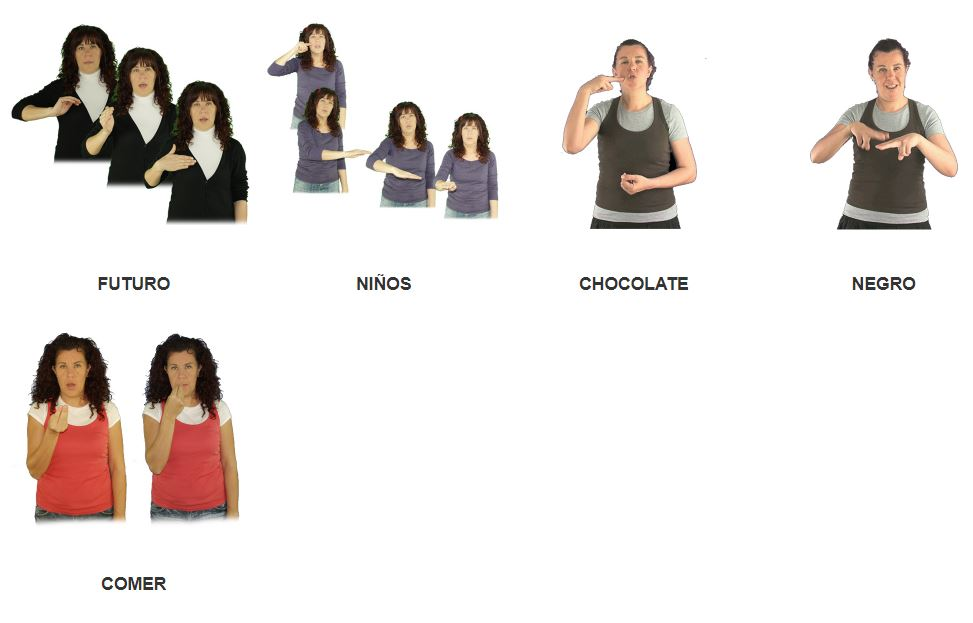
\includegraphics[width=1\textwidth]{Imagenes/Fuentes/Apendices/E15.jpg}
		\caption{Verbal tense and possessive sentence in SSL translated by Text2LSE }
		\label {fig: AP_E15_cap8_in}
	\end{figure}
	
	
	\item \textbf{Changes in possessive determinants:} The determinants that indicate possession are replaced by personal pronouns, as it can be seen in Figure ~\ref {fig: AP_E17_cap8_in}.
	
	\begin{figure}[]
		\centering
		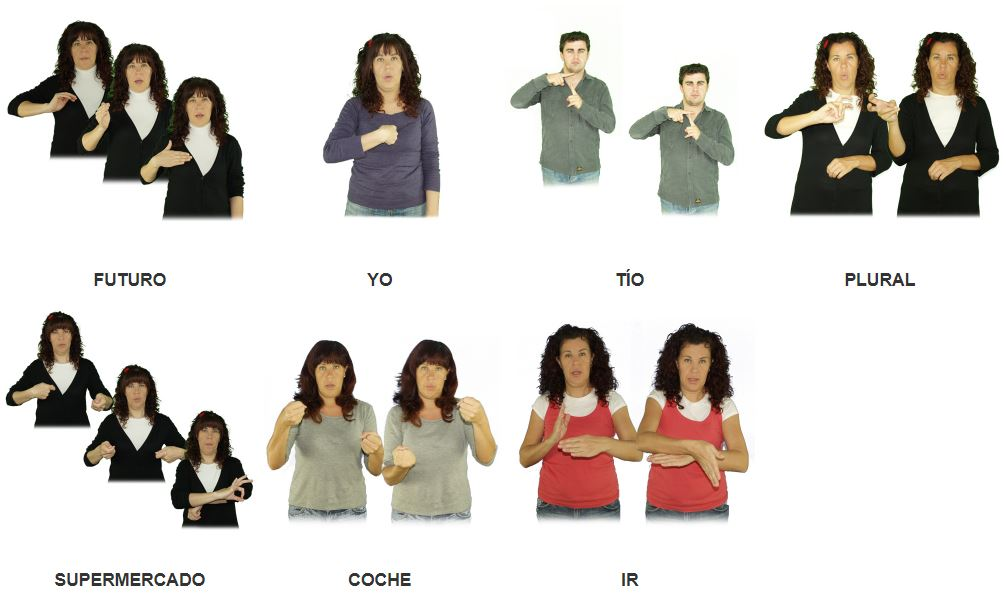
\includegraphics[width=1\textwidth]{Imagenes/Fuentes/Apendices/E17.jpg}
		\caption{Verbal tense and possessive sentence in SSL translated by Text2LSE }
		\label {fig: AP_E17_cap8_in}
	\end{figure}
	
	\item \textbf{Gender and number}: The tool detects the gender and number of each noun and shows the signs ``PLURAL'' in the case of the number or woman (``MUJER'') in the case of gender, as it can be seen in Figure  ~\ref {fig: AP_E16_cap8_in}.
	
	\begin{figure}[]
		\centering
		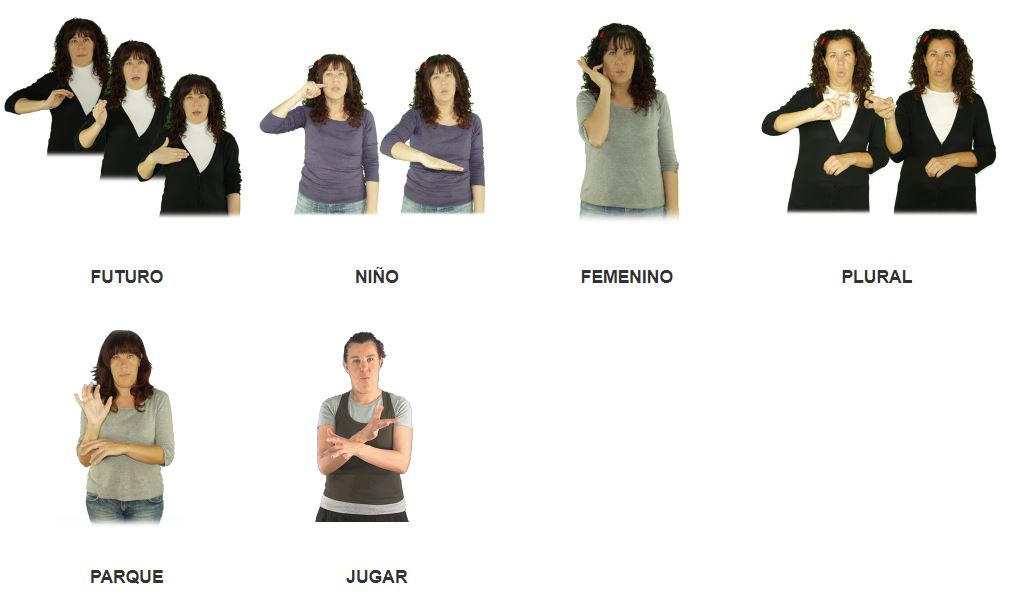
\includegraphics[width=1\textwidth]{Imagenes/Fuentes/Apendices/E16.jpg}
		\caption{Sentence with gender and number in SSL translated by Text2LSE}
		\label {fig: AP_E16_cap8_in}
	\end{figure}
	
	\item \textbf{Adjectives}: It detects every adjective in the sentence and turns them to singular masculine, such as Figure ~\ref {fig: AP_E2_cap8_in}.
	
	\begin{figure}[]
		\centering
		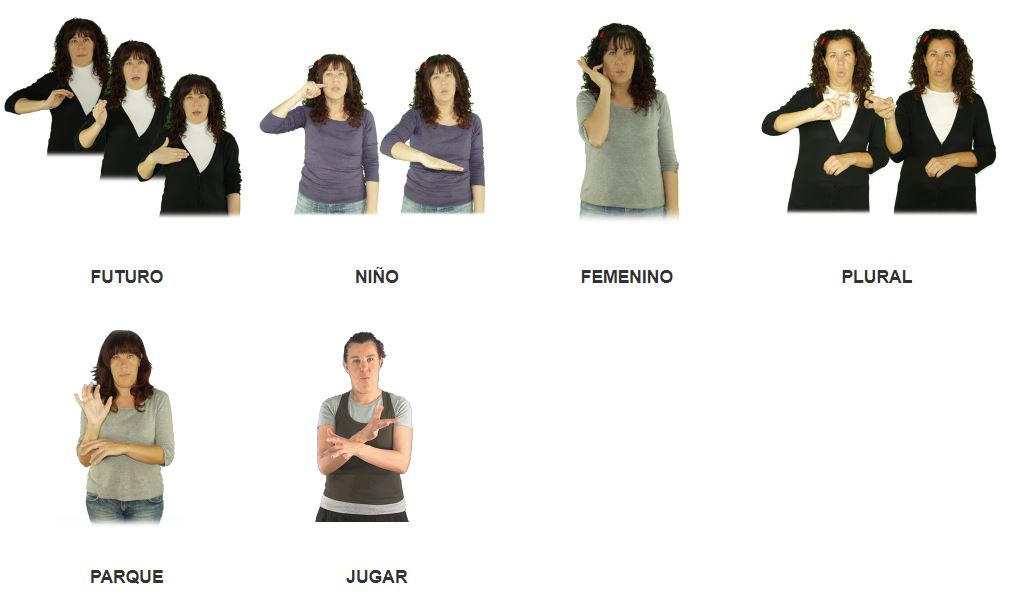
\includegraphics[width=1\textwidth]{Imagenes/Fuentes/Apendices/E16.jpg}
		\caption{Sentence with adjectives in SSL translated by Text2LSE}
		\label {fig: AP_E2_cap8_in}
	\end{figure}
	
	
\end{itemize}

Although there is a lot of work to be done, we would like to highlight the fact that at the beginning of this project an analysis was made to similar applications on the market, but we did not find any application that carried out text translations to SSL in real time, so we can say that, though the result is not perfect, this work provides a good basis for the translation from natural language to Spanish Sign Language. \\

Another important aspect of the work that we developed was creating a public API\footnote{\url{https://holstein.fdi.ucm.es/tfg-text2lse/}} with the developed web services, in such a way that it is easy to use in other projects.\\ 

Apart from translation, the purpose was also to create an application with an intuitive interface that is accessible to everyone from any device. The initial plan was to carry out an evaluation of the interface with real users, but due to the Covid-19 crisis such an evaluation was not possible. Still, taking into account the opinions of the tutors in this regard and following their design advice, we believe that the interface is simple and intuitive and we meet the objective set.\\

The development of Text2LSE has allowed us to apply a great amount of knowledge acquired during the Computer Engineering Degree in a large project with a social utility, not only in the academic field. Some subjects that have been very important to carry out this project are:

\begin{itemize}
	
	
	\item \textbf{Web applications: } This subject helped us when doing the Front-end, since it provided us with great knowledge about web development with HTML, CSS and Javascript, which was very useful for this project.
	
	\item \textbf{Programming Technology:} Thanks to this subject we learned to program a project in Java. Although the project is programmed in Python, the important thing about this course is that it provided us with great knowledge when programming, so learning a new language like Python was not very complicated.
	
	\item \textbf{Algorithmic Data Structure}: What helped us the most in this subject was knowing how to use recursion when programming, since it has been a fundamental pillar in the NLP.
	
	\item \textbf{Ethics, Legislation and Profession}: This is a subject that taught us how to use the licenses with which to protect our work, as well as learning to use free software and to  correctly reference all the information used in the project.
	
	
\end{itemize}

Also the project allowed us to gain new knowledge that was not taught in the degree, such as: Web Services, Proxies, NLP, Python...


\section{Future Work}
\label{cap8:sec:TrabajoFuturo_in}

With the aim of improving some functionalities of the Text2LSE tool in order to obtain a more complete application and with greater coverage, we think that the following could be marked as future work:

\begin{itemize}
	
	
	\item \textbf{Proper names translation:} In the SSL, proper names can be translated using either the sign of each letter to complete the name or use a proper sign that defines the person. Currently, the application detects the proper name but cannot find a translation, since there are no images or videos for that name, as it can be seen in Figure ~\ref{fig: AnaAlta_in}. The solution would be to use the sign of each letter of the proper name, as it can be seen in Figure ~\ref{fig: NombreBien_in}
	
	\begin{figure}[]
		\centering
		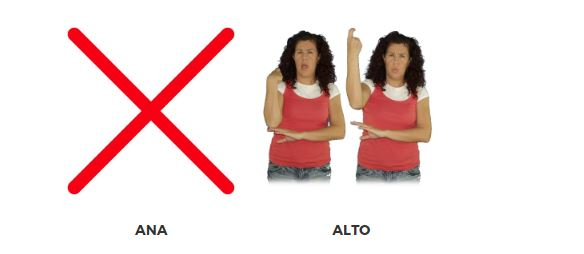
\includegraphics[width=1\textwidth]{Imagenes/Fuentes/Conclusiones/AnaAlta.jpg}
		\caption{Example of bad translation of a proper name made by Text2LSE }
		\label {fig: AnaAlta_in}
	\end{figure}
	
	
	\begin{figure}[]
		\centering
		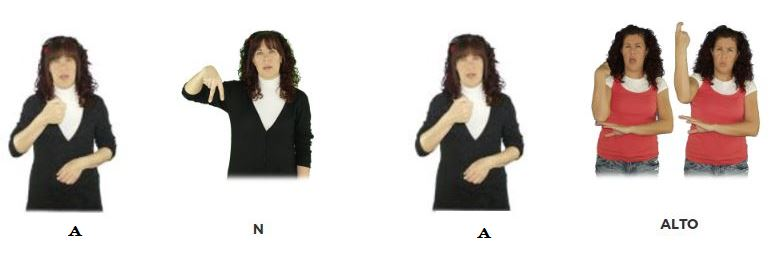
\includegraphics[width=1\textwidth]{Imagenes/Fuentes/Conclusiones/NombreBien.jpg}
		\caption{Example of a good translation of a proper name made by Text2LSE}
		\label {fig: NombreBien_in}
	\end{figure}
	
	
	\item \textbf{Improving Gender and Number:} As stated in section \ref{cap6:sec:An�lisis de los Resultados}, the detection of when to add the sings that indicate femenine or plural would be an improvement, since sometimes it is not necessary to add then, for example in the word ``rampas'' whose translation would be the sign \textit{``RAMPAS''} (Figure ~\ref {fig: rampas_in}). However, the application translates it as ``RAMPAS + FEMENINO + PLURAL'', as it can be seen in Figure ~\ref {fig: rampasMal_in}
	
	\begin{figure}[]
		\centering
		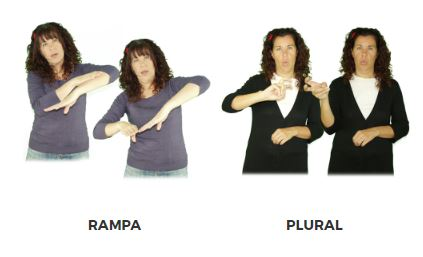
\includegraphics[width=0.6\textwidth]{Imagenes/Fuentes/Conclusiones/rampas.jpg}
		\caption{Correct translation of the word ``rampas'' by Text2LSE}
		\label {fig: rampas_in}
	\end{figure}
	
	\begin{figure}[]
		\centering
		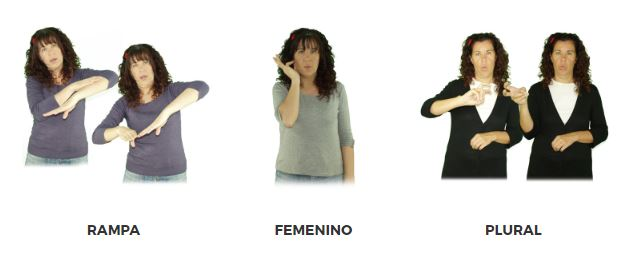
\includegraphics[width=1\textwidth]{Imagenes/Fuentes/Conclusiones/rampasMal.jpg}
		\caption{Incorrect translation of the word ``rampas'' by Text2LSE}
		\label {fig: rampasMal_in}
	\end{figure}
	
	\item \textbf{Adding denial:} Currently, the rule system does not contemplate negative sentences, so it would be a great advance to add a rule that allows a negative sentence to be correctly translated in SSL.
	
	\item \textbf{Recognition of compound verbal tenses:} The application is currently not capable of recognizing compound tenses, such as ``han comido'' or ``estaban comiendo'', so it would be important to expand the NLP part of Text2LSE so that these types of verbs are correctly translated. In Figure ~\ref {fig: hanComidoPanMal_in} it can be seen that our application tries to translate the verb ``to have'' and finds no result. The correct option would be the one in Figure ~\ref {fig: hanComidoPanBien_in}
	
	\begin{figure}[]
		\centering
		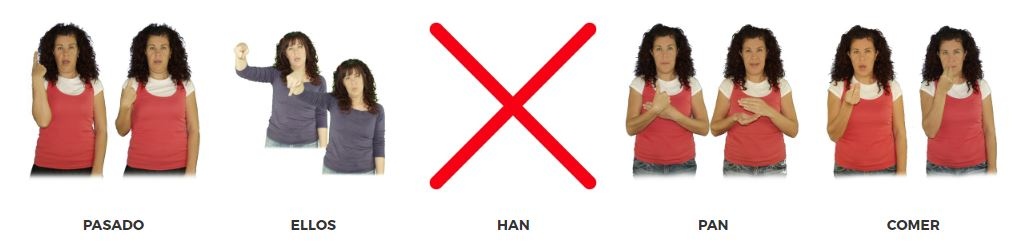
\includegraphics[width=1\textwidth]{Imagenes/Fuentes/Conclusiones/hanComidoPanMal.jpg}
		\caption{Example of bad translation of compound times made by Text2LSE}
		\label {fig: hanComidoPanMal_in}
	\end{figure}
	
	\begin{figure}[]
		\centering
		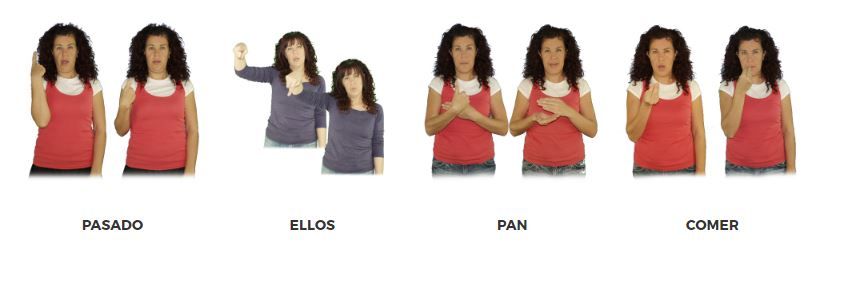
\includegraphics[width=1\textwidth]{Imagenes/Fuentes/Conclusiones/hanComidoPanBien.jpg}
		\caption{Example of good translation of compound times made by Text2LSE}
		\label {fig: hanComidoPanBien_in}
	\end{figure}
	
	\item \textbf{Sentences that do not requiere NLP:} It contemplates the identification of sentences made that have their own sign and do not require a word-by-word translation. For example, the sentence ``Secar el pelo'' is translated with a single sign, as it can be seen in Figure ~\ref {fig: pelosecar_in}. However, our application performs the translation as if it were a normal sentence (See Figure ~\ref {fig: SecarPeloMAL_in})
	
	\begin{figure}[]
		\centering
		
\includegraphics[width=0.4\textwidth]{Imagenes/Fuentes/Conclusiones/pelosecar.jpg}
		\caption{Sign in SSL for the phrase ``Secar el pelo'' }
		\label {fig: pelosecar_in}
	\end{figure}
	
	\begin{figure}[]
		\centering
		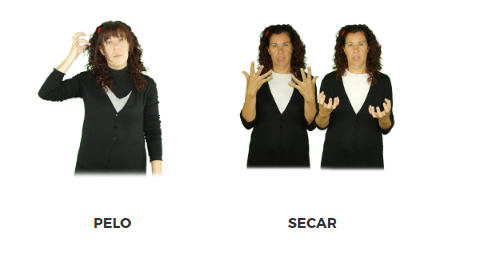
\includegraphics[width=1\textwidth]{Imagenes/Fuentes/Conclusiones/SecarPeloMAL.png}
		\caption{Sign in SSL for the phrase ``Secar el pelo'' made by Text2LSE}
		\label {fig: SecarPeloMAL_in}
	\end{figure}
	
	\item \textbf{Translation of compound sentences:} The current version of Text2LSE allows for the translation of simple sentences, but it does not translate compound sentences, such as ``Los ni�os fueron al parque para jugar con sus amigos'' In this sentence, it can be seen that there are two simpler well distinguished sentences: ``Los ni�os fueron al parque'' and ``(Los ni�os) jugar con sus amigos''. Developing a set of rules to translate compound sentences would be an improvement.
	
	
	\item \textbf{Improvement in the System NLP:} The NLP system is used in this project through a system of rules using the Spacy tool. This system is not capable of translating sentences that are not contemplated in the previously programmed rules. Changing the rule-based system to one based on machine learning, which is capable of learning by itself in order to translate any sentence would be an interesting and very important improvement.
	
	
\end{itemize}


\end{otherlanguage}





%-------------------------------------------------------------------



